%!TEX root = ../projektplan.tex
\chapter{Infrastruktur}

\section{Hardware}
Als Entwicklungsgeräte werden die einzelnen Notebooks der Projektmitarbeiter eingesetzt. Das Testing der Webapplikation soll ebenfalls auf den Geräten ausgeführt werden. Gehostet wird die Applikation auf einer virtuellen Maschine mit Windows Server 2012. Eingesetzt wird dafür die Infrastruktur der HSR.

\section{Software / Tools}
Für die Entwicklung wird Visual Studio 2013 eingesetzt. Mittels Visual Studio Online wird die Sourcecodeverwaltung vorgenommen und ebenfalls als Build-Server eingesetzt. Für die Datenpersistenz wird ein Microsoft SQL Server eingesetzt. Zum Hosting der Webapplikation setzen wir einen IIS Webserver ein.
\begin{figure}[h]
    \centering
    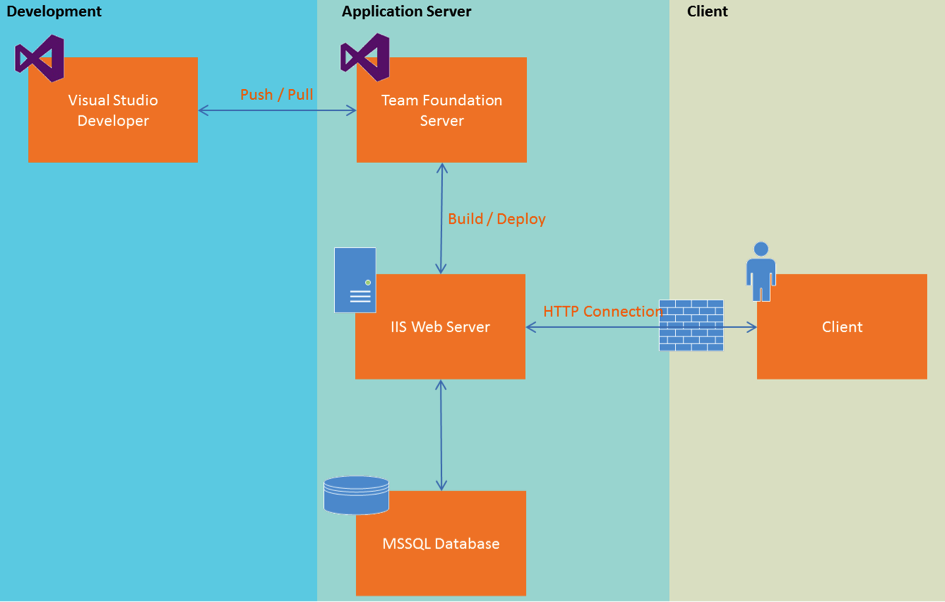
\includegraphics[width=0.8\textwidth]{content/images/infrastruktur.png}
    \caption{Infrastruktur}
\end{figure}

\subsection{Tools}	
		\begin{table}[H]
		    \tablestyle
		    \tablealtcolored
		    \begin{tabularx}{\textwidth}{l X}
		        \tableheadcolor
		            \tablehead Bezeichnung &
		            \tablehead Erläuterung \tabularnewline
		        \tablebody
		        \textbf{Visual Studio 2013} &
		        	Entwicklungsumgebung, Quellcodeverwaltung
		            \tabularnewline
		        \textbf{JetBrains ReSharper 8.1} &
		            Toolset für Visual Studio 2013, Test Coverage, Coding Standards
		            \tabularnewline
		        \textbf{Astah Community 6.8.0} &
		            Erstellung von Diagrammen
		            \tabularnewline
		        \textbf{Visual Studio Online} &
		            Ablage der Codebase mittels TFS, Builds
		            \tabularnewline
		        \textbf{ISS} &
		            Webserver für Applikation
		            \tabularnewline
		        \textbf{MSSQL} &
		            Datenbank für Persistenz der für Applikation
		            \tabularnewline
		        \textbf{SQL Management Studio 2012} &
		            Zugriff und Verwaltung der MSSQL Datenbank
		            \tabularnewline
		        \textbf{\LaTeX} &
		            Textsetzung für Dokumentationen
		            \tabularnewline
		        \textbf{Git / GitHub} &
		            Ablage der Dokumentationen 
		            \tabularnewline
		        \textbf{\href{http://www.minutes.io}{minutes.io}} &
		            Tool für Besprechungsnotizen
		            \tabularnewline
		        \tableend
		    \end{tabularx}
		    \caption{Verwendete Tools}
		\end{table}